\section{Data}
\label{sec:data}

We explore the behavior of metrics on mock classification probabilities with isolated strengths and weaknesses as well as realistic mock classification probabilities from a publicly available lightcurve catalog.
Throughout this paper, \textit{data} always refers to mock classification submissions to \plasticc, not the \plasticc\ lightcurves; no lightcurves were simulated, viewed, or classified in the preparation of this paper.

Our data is in the form of catalogs of $N$ posterior probability vectors $p(m \mid d_{n}, D, \mathcal{C})$ over $M$ classes with labels $m$ conditioned on each observed lightcurve $d_{n}$, the training set $D$, and some parameters $\mathcal{C}$ concerning the behavior of the classifier.
We motivate $\mathcal{C}$ here before deferring its detailed explanation to later in Section~\ref{sec:mockdata}.
If a mock classifier produced $p(m \mid d_{n})$, it would take solely the lightcurve and produce a posterior over classes.
Since such a situation involves no information besides the lightcurve $d_{n}$, every classifier would produce identical classification submissions $p(m \mid d_{n})$.
Including the training set $D$ would not remedy the problem, as every classifier has access to the same training set and so would still have no way to produce different classification submissions $p(m \mid d_{n}, D)$.
Thus there must be some other parameters $\mathcal{C}$ that are specific to each classifier and contribute to the mock classification posteriors it produces.
We describe below the way in which mock data is synthesized and return to the classifier parameters $\mathcal{C}$ later.

\begin{figure}
	\begin{center}
    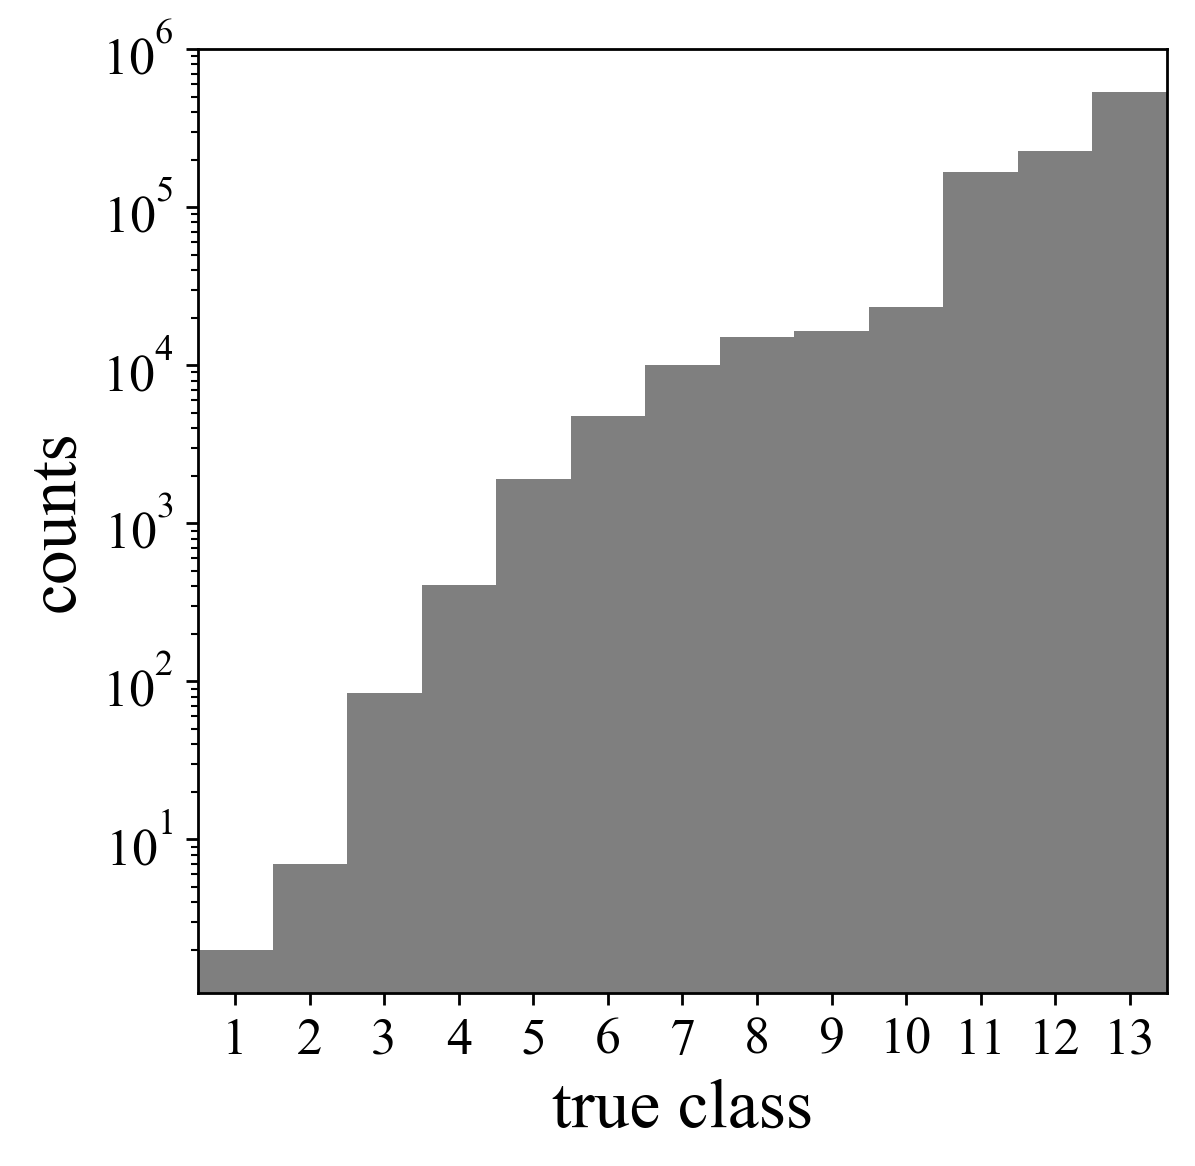
\includegraphics[width=0.49\textwidth]{./fig/complete_counts.png}
		\caption{The number of objects in a given class as shown as a function of class label, in increasing class size.
		The true classes are logarithmically distributed.}
		\label{fig:classdist}
	\end{center}
\end{figure}

As is anticipated of the real \lsst\ dataset, we use class populations that are logarithmically distributed such that they span many orders of magnitude.
%We then take $M$ draws $u_{m} \sim \mathcal{U}(0, 1)$ from the standard continuous uniform distribution and establish a discrete probability distribution $p(m) = b^{u_{m}}\ Z^{-1}$ where $Z = \sum_{m} b^{u_{m}}$, i.e. such that $\sum_{m=1}^{M} p(m) = 1$.
We take $M$ draws $u_{m'} \sim \mathcal{U}(0, 1)$ from the standard continuous uniform distribution.
These coefficients $u_{m'}$ define the discrete probability distribution $p(m') = b^{u_{m'}} / \sum_{m'} b^{u_{m'}}$ for each class $m'$ such that $\sum_{m'=1}^{M} p(m') = 1$.
% was the b in 10^b really related to the b above? This was not clear. \aim{Yes, it is the same b}
From $p(m')$ we draw $N = 10^{b}$ instances $\{m'_{n}\}$ of a true class $m'$ for each lightcurve $n$ in the catalog.
The true class membership distribution of our tests with $M = 13$ and $b = 6$ is shown in Figure~\ref{fig:classdist}.
Though the class labels for \plasticc\ are expected to be randomized, we artificially order our mock class labels by their prevalence for ease of visual interpretation.
Once the true classes have been set, mock classification probabilities for each class are derived using the procedure described in Section~\ref{sec:mockdata}.

\subsection{Mock classification schemes}
\label{sec:mockdata}

In order to observe metric performance on different classification schemes, we develop archetypical mock classifiers, devised to produce generic responses to a classification challenge without any interaction with lightcurves, images, or any other test set or training set from any challenge.
We use these mock classifiers to investigate how the performance under each metric changes in the presence of certain types of failure modes, or \textit{systematics}.
A robust metric should not reward classification schemes that display these systematic effects.
% In other words, we want a metric that deters ``gaming the system'' as much as possible.
%The cases of this section are devised to test if a metric is congruent with our intuitive understanding of what constitutes a good classifier, that it should not reward classifications suffering from the most concerning failure modes, which we will refer to as \textit{systematics} throughout the paper.
%% TODO change systematics to symptoms?
%Our impressions of systematics can be seen as reflections of the conditional probability matrix, a familiar metric of deterministic classification \citep{2012PASP..124.1175B}.

The archetypical systematics can be seen as modifications to the confusion matrix, a familiar measure of deterministic classification \citep{bloom_automating_2012}.
The confusion matrix is an $M \times M$ table of observed counts (or, if normalized, rates) of pairs of estimated class labels $\hat{m}$ (columns) and true classes $m'$ (rows) computed after a deterministic classification has been performed on some data set with $N$ objects.

Under a binary deterministic classification between positive and negative possibilities, it is natural to count the numbers of true positives $\mathrm{TP}$, false positives $\mathrm{FP}$ (Type 1 error), true negatives $\mathrm{TN}$, and false negatives $\mathrm{FN}$ (Type 2 error), which can be turned into rates relative to the true numbers of positive and negative instances; these rates may serve as building blocks for more sophisticated metrics of multi-class deterministic classifiers addressed in Section~\ref{sec:methods}.
Though probabilistic classifications are not compatible with the confusion matrix, regardless of normalization, we design tests around proposed normalized confusion matrices exhibiting various symptoms that we anticipate being problematic for \lsst.

Under a deterministic classification scheme with a normalized confusion matrix with elements $p(\hat{m}, m')$, an object with true class $m'$ would have an assigned class $\hat{m}$ drawn from $p(\hat{m} \mid m') = p(\hat{m}, m') / p(m')$, via Bayes' Rule.
We note that the elements of the confusion matrix have values of $N p(\hat{m}, m')$ and that $p(m') = N_{m'} / N$, where $N_{m'}$ is the number of true members of class $m'$, must be known in order to produce a confusion matrix.
We can thus easily obtain classification posteriors $p(\hat{m} \mid m')$ to use as the basis for classification probability submissions resulting from a confusion matrix.

Given its provenance, we refer to the matrix $\mathbb{C}$ comprised of $p(\hat{m} \mid m')$ as the \textit{conditional probability matrix} (CPM).
Without loss of generality, we can decompose $\mathbb{C}$ under some basis functions of parameters $\mathcal{C}$, the same as those introduced above in the definition of a classification posterior $p(m \mid d_{n}, D, \mathcal{C})$.
The CPM $\mathbb{C}$ thus defines the behavior of a classifier.

Since we believe the lightcurves contain information about the true class (an assumption that underlies classification as a whole), we can use the appropriate row $\mathbb{C}_{m'_{n}} = p(\hat{m} \mid m', \mathcal{C})$ of the CPM $\mathbb{C}$ as a proxy for $p(m \mid d_{n}, D, \mathcal{C})$, without directly classifying lightcurves themselves, which enabled this paper to be written without any knowledge of the \plasticc\ dataset's simulation nor validation.

To emulate the effect of natural variation of information content in different lightcurves, we generate a posterior probability vector $\vec{p}(m \mid m', \mathbb{C})$ by taking a Dirichlet-distributed draw
\begin{eqnarray}
  \label{eq:cmtoprob}
  \vec{p}(m \mid d_{n}, D, \mathcal{C}) &\sim& \mathrm{Dir}[\mathbb{C}_{m'_{n}} \delta]
	 % \frac{\mathrm{Gamma}(\mathbb{C}_{m_{n}'} \delta)}{\sum_{m'} \mathrm{Gamma}(\mathbb{C}_{m'} \delta)}
\end{eqnarray}
about $\mathbb{C}_{m'_{n}}$, with a small nonnegative perturbation factor $\delta = 0.01$.
In this way, the posterior probability vector has an expected value equal to the appropriate row in the CPM, with a variance set by $\delta$.
% \begin{eqnarray}
%  \label{eq:gamma}
%  \Gamma(\alpha) &=&
% \end{eqnarray}
We impose one restriction in addition to the normalization factor of Equation~\ref{eq:cmtoprob}, namely that all elements of $p(m \mid d_{n}, D, \mathcal{C})$ exceed $10^{-8}$, to ensure numerical stability in light of the limitations of floating point precision.

% TODO: letters for panels, refer to them in text
\begin{figure*}
	\begin{center}
    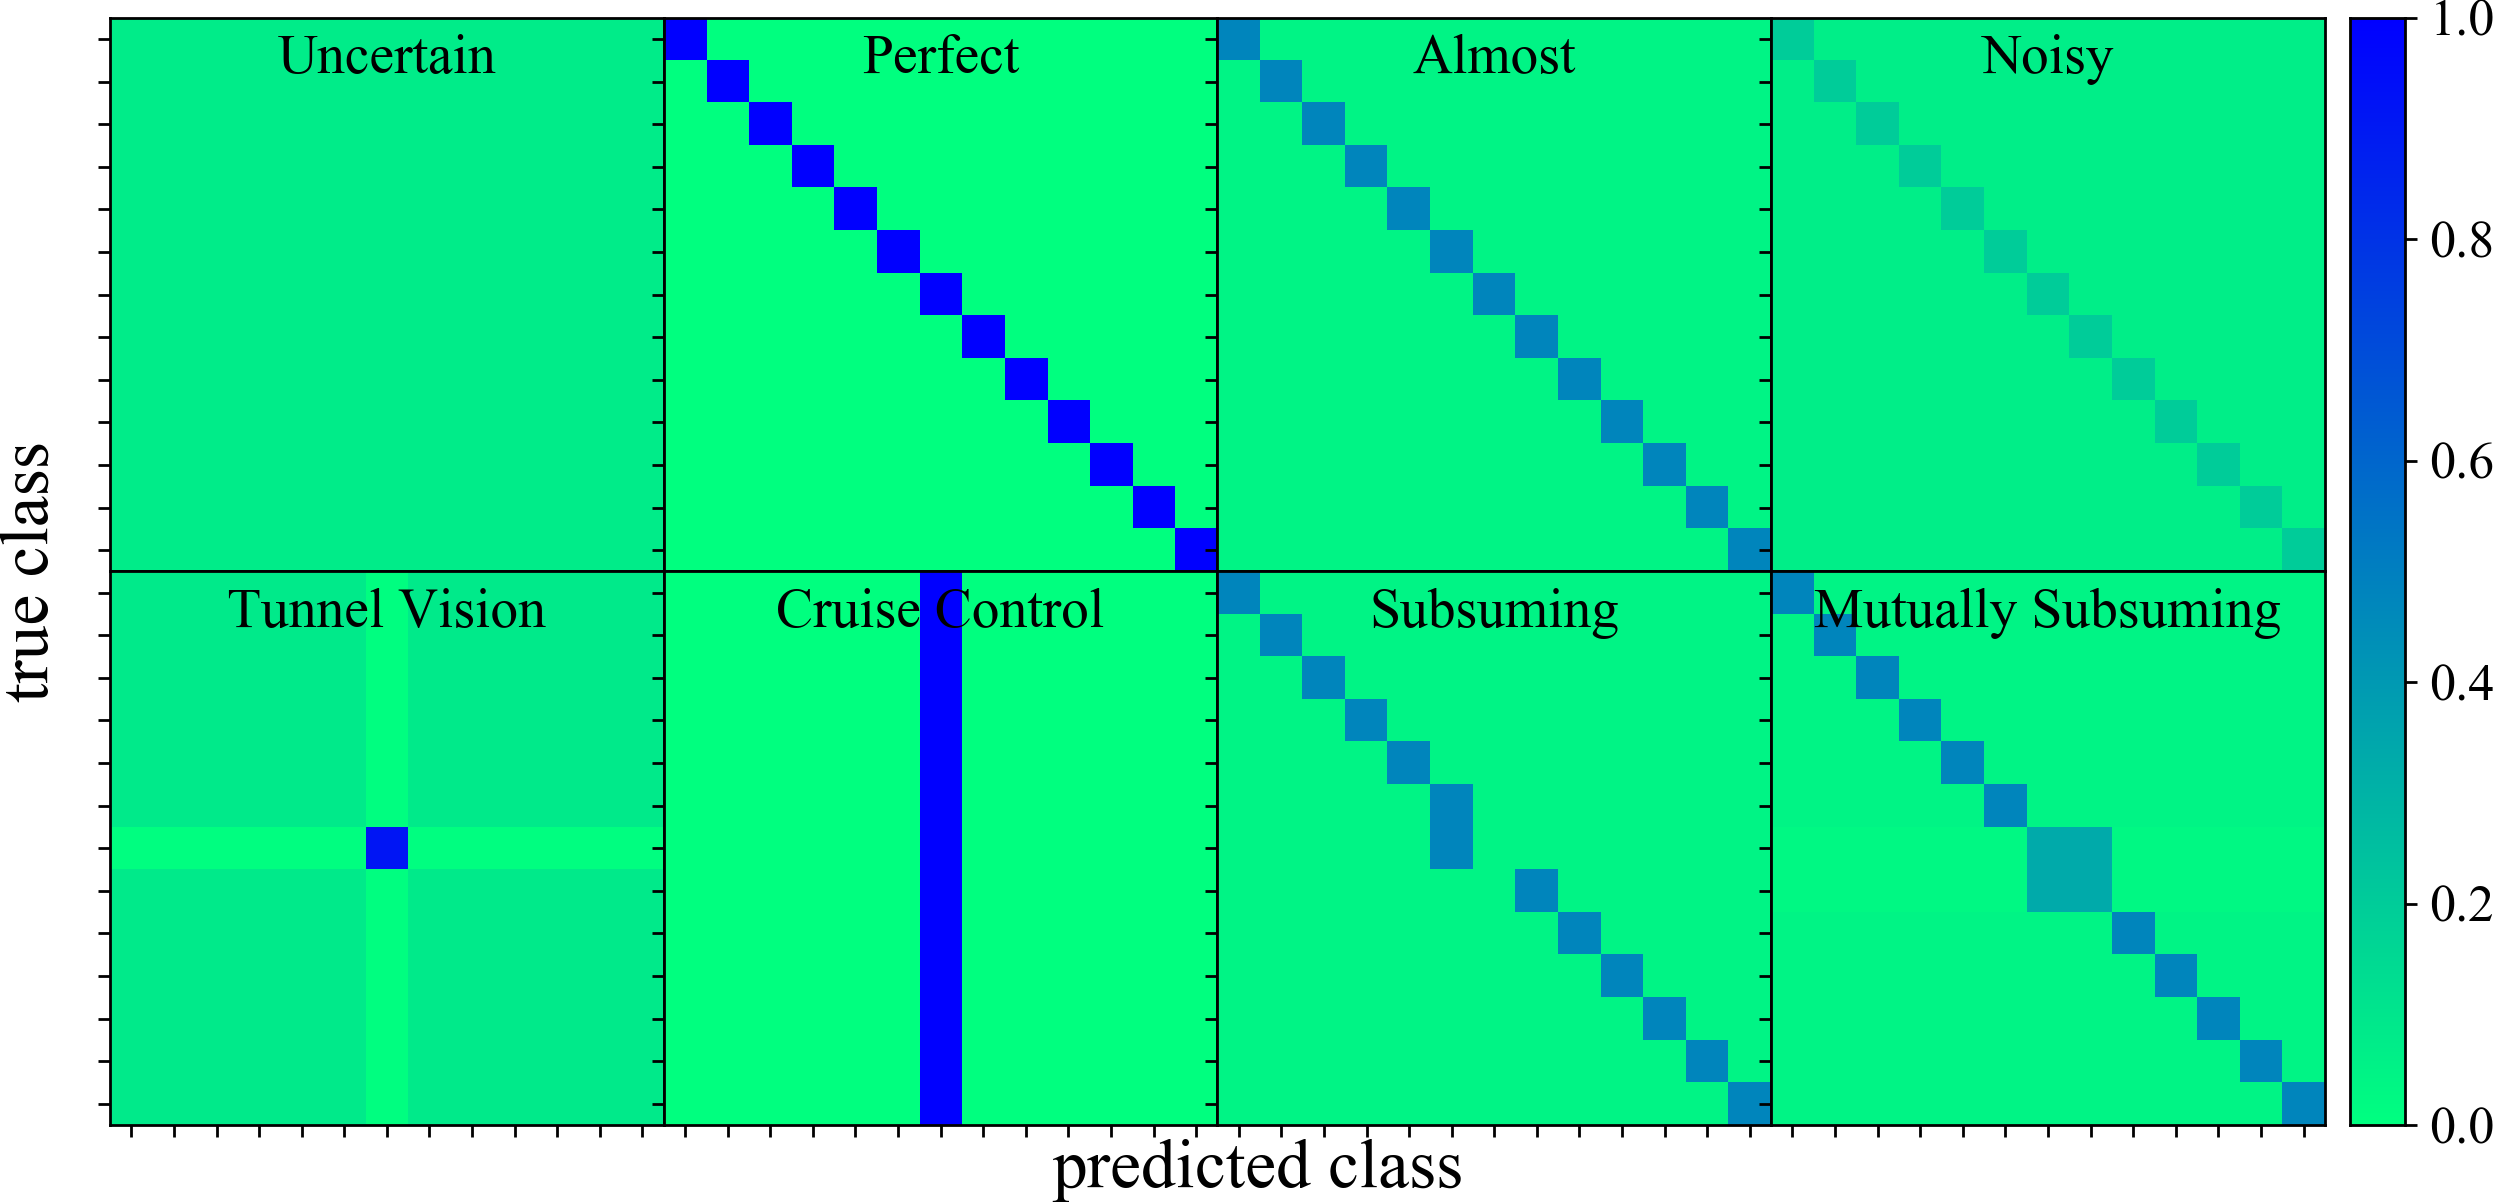
\includegraphics[width=0.8\textwidth]{./fig/all_sim_cm.png}
		\caption{Conditional probability matrices for eight mock classifiers.
		Top row:
		the uncertain classifier's uniform CPM;
		the perfect classifier's identity CPM;
		the almost perfect classifier's CPM, a linear combination of one part uniform and four parts identity;
		the noisy classifier's CPM, a linear combination of one part uniform and two parts identity.
		Bottom row:
		the tunnel vision classifier's CPM is uniform except at the row and column corresponding to one class, where it takes the values of the identity matrix;
		the cruise control classifier's CPM, which has the every row equal to a particular row of the identity;
		the subsuming classifier's CPM, which has two or more rows equal to one another;
		the mutually subsuming classifier's CPM, a symmetric case of the subsuming classifier.
		The top row shows CPMs that serve as unbiased control cases.
		The CPMs of the bottom row represent concerning systematics that we would like to ensure are not rewarded by the \plasticc\ metric.
		% The left panels show uncertain (top) and perfect (bottom) classifications, while the second panel from the left shows the almost perfect (top) and unbiased but noise (bottom) classifications. The third panel from the left illustrate the perfect classifications that generate Type 1 (False Positive) and Type 2 (False Negative) errors for one class and uniform for all others (the `tunnel classifier', top row), while the bottom row illustrates the classification where all objects are assigned to the same class (the `cruise' classifier). Finally, the panels on the far right show classifications where one class is consistently assigned to another class (subsumed to, top row), and where one consistently assigns another class to one particular class (subsumed from, bottom row). Such classifications arise when one is optimising for a particular science case (e.g., one might prioritize a tunnel classification scheme), or where one object is considered much more `valuable' to classify than others (in which case one would employ a cruise classification scheme.)
		}
		\label{fig:mock_cm}
	\end{center}
\end{figure*}

\begin{figure}
	\begin{center}
		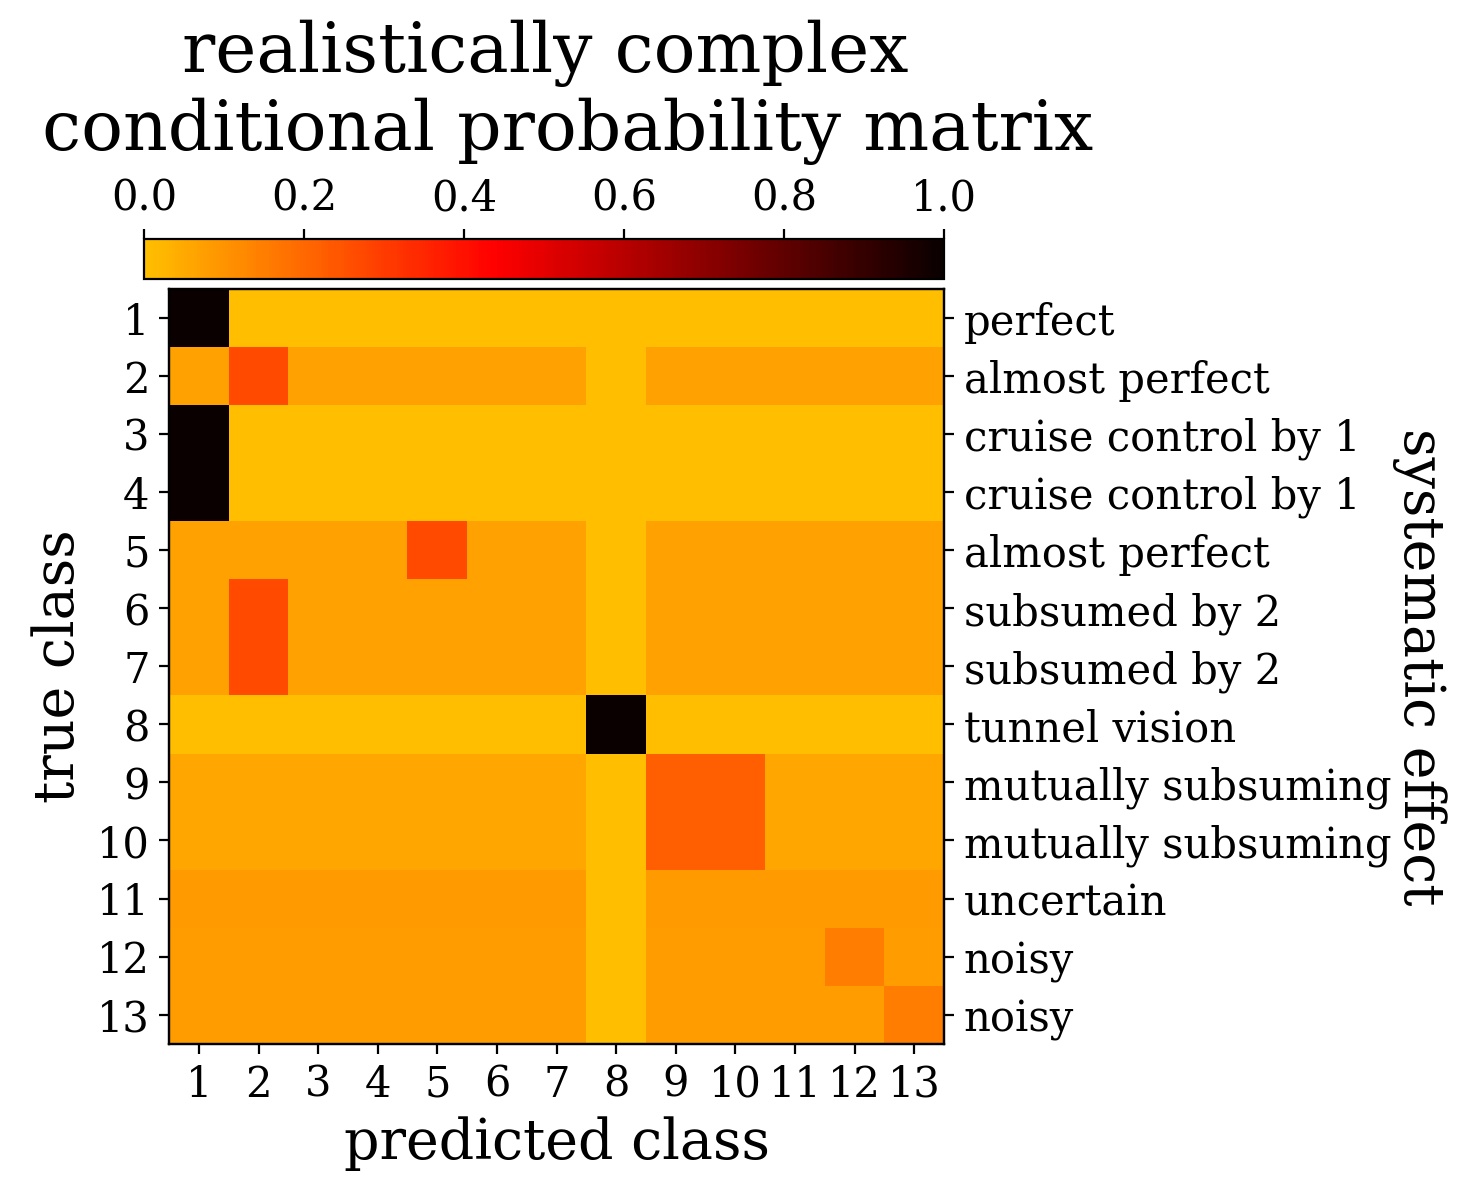
\includegraphics[width=0.49\textwidth]{./fig/combined.png}\\
    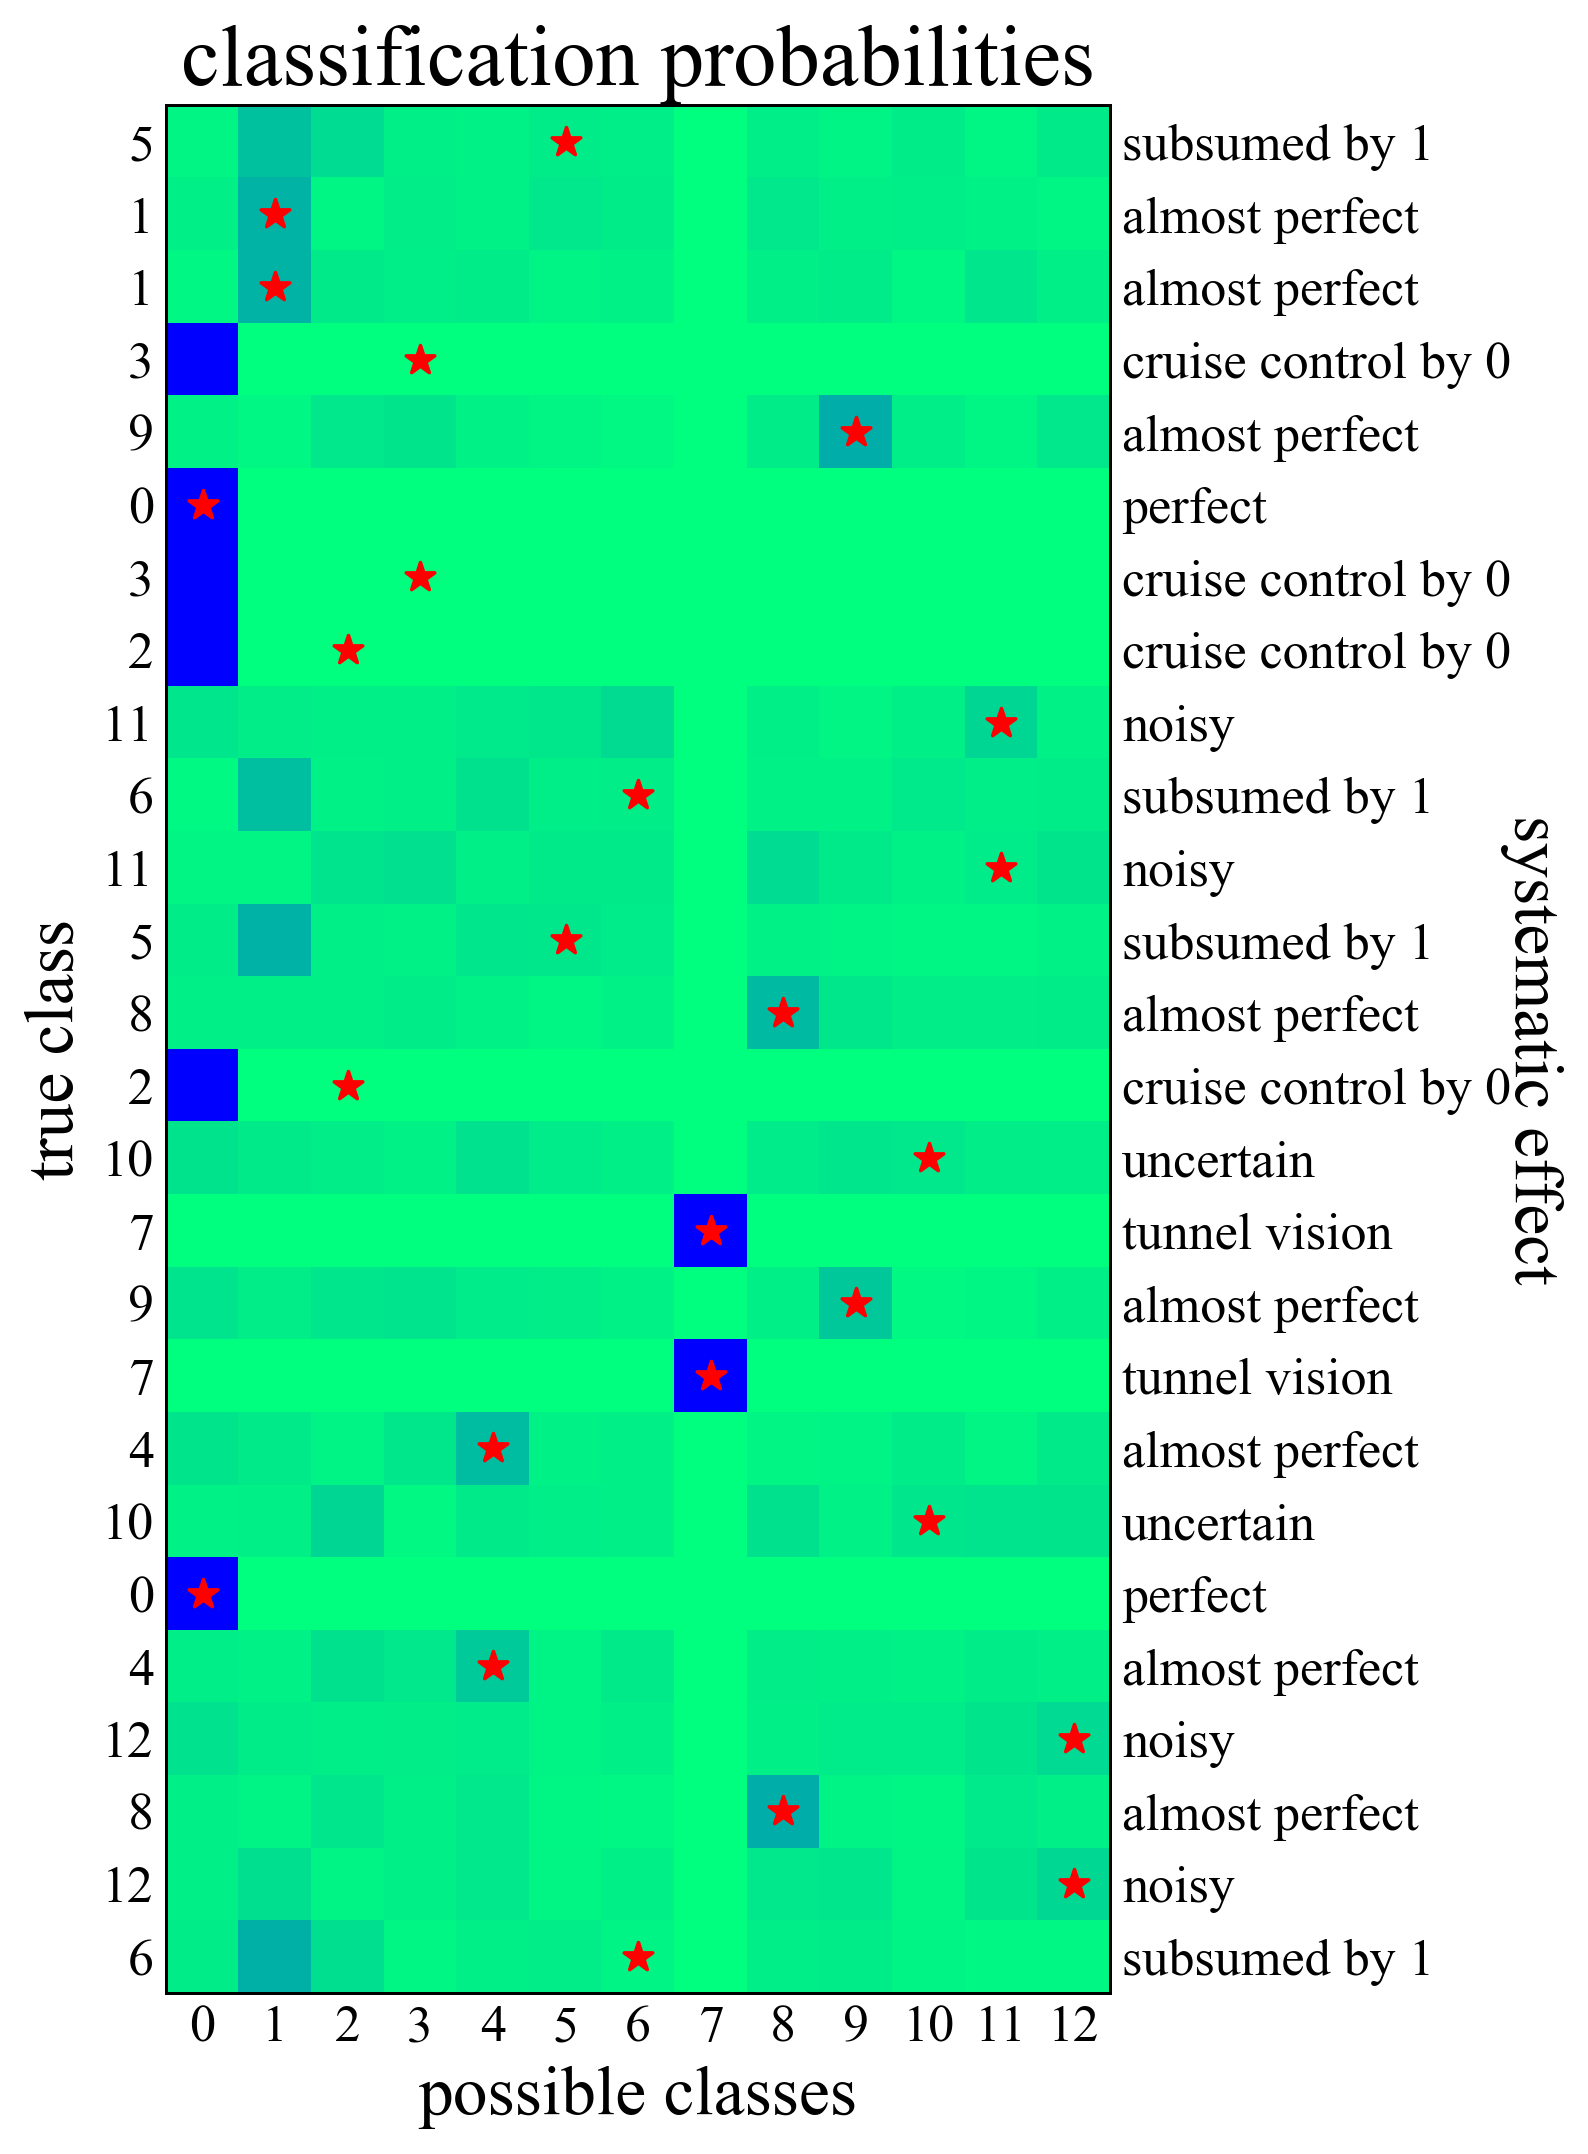
\includegraphics[width=0.49\textwidth]{./fig/examples.png}
		\caption{A realistically complex conditional probability matrix and classification posteriors drawn from it.
		Top: A realistic classifier's conditional probability matrix, characterized by a combination of systematics described on the right.
		Bottom: Classification posteriors drawn from the conditional probability matrix above, with their true class indicated by a red star as well as on the left.
		The text on the right describes the true class as in the top panel.
		}
		\label{fig:mock_probs}
	\end{center}
\end{figure}

We consider eight mock classifiers, each characterized by a single systematic affecting their CPM.
Figure~\ref{fig:mock_cm} shows the CPMs corresponding to each systematic considered, discussed in detail below.
An example of a composition thereof is given in Figure~\ref{fig:mock_probs}, along with examples of the mock classification posteriors drawn from it.

For each case, we address:
\begin{enumerate}
  \item What characteristic behavior defines this classifier?
  \item Under what conditions does this behavior arise in real classifications?
  \item What are our expectations of and desires for response of the metric to this archetypical classifier?
\end{enumerate}

\subsubsection{Uncertain classification}
\label{sec:uncertaindata}

An entirely uniform CPM $\mathbb{U}$ (leftmost top panel of Figure~\ref{fig:mock_cm}) would correspond to uniform random guesses for deterministic classification, but, in accordance with Equation~\ref{eq:cmtoprob}, the classification posteriors are perturbations away from a uniform distribution across all classes.
The peak values of these classification posteriors will correspond to uniform random classifications, with $p(m' \mid d_{n}, D, \mathcal{C}_{\mathbb{U}}) \approx M^{-1}$.
We can consider the \textit{uncertain} classifier as an experimental control for the worst possible classification scheme, bearing in mind that if classifications were anticorrelated with true classes, the experimenter could simply reassign the classification labels to improve performance under any metric.

\subsubsection{Accurate classification}
\label{sec:accuratedata}

The \textit{perfect} classifier has a diagonal CPM $\mathbb{I}$ (left-center top panel of Figure~\ref{fig:mock_cm}), which would correspond to deterministic classifications that are always correct.
In terms of probabilistic classifications, a perfect result would be a classification posterior with 1 for the true class and 0 for all other classes.
In accordance with the classification posterior synthesis scheme of Equation~\ref{eq:cmtoprob}, the class with maximum probability is almost always still the true class, and indeed with $N \sim 10^{6}$ and $\delta = 0.01$, this is always true.
This case is also a control, in that \plasticc\ would not be necessary if we believed the perfect classifier were potentially achievable.

In addition to a perfect classifier, we test linear combinations $\mathbb{C} = (s + 1)^{-1} \left(s\mathbb{I} + \mathbb{U}\right)$ of the perfect and uncertain CPMs where the contribution of the perfect classifier is greater than that of the uncertain classifier by a factor of $s > 0$.
Deterministic classifications drawn from such a CPM would be correct $s$ times as often as they take any one wrong label, and the incorrect labels would be uncorrelated across classes.
The classification posteriors drawn from such CPMs would have some probability at classes other than the true class, but virtually all would still have their peak value at their true class.
% While $s$ would realistically be expected to vary for each class, we do not conduct a systematic investigation of this possibility at this time, and instead fix $s$ as constant for any given mock classifier.
We consider the case of the \textit{almost perfect} classifier with $s=4$ (right-center top panel of Figure~\ref{fig:mock_cm}) and the \textit{noisy} classifier with $s=2$ (rightmost top panel of Figure~\ref{fig:mock_cm}).

A classifier with different accuracy for each class may be considered a systematic in its own right.
An extreme example of such a classifier could be one with perfect classification performance on one class and uncertain classification on all others.
This classifier's CPM would be uniform except for one row, which would take a value of unity on the diagonal and zero elsewhere; if the classifier were also resilient against Type 1 errors, the CPM would also take zeros along the column in question, aside from the value of unity on the diagonal.
For many specific science applications, this type of classifier is desirable, but given the balancing of science cases within \lsst, we take a more measured approach and require that the \plasticc\ metric serve the needs of those who study a wide variety of classes for different purposes.
Hence, from the perspective of \plasticc, we seek a metric that disfavors the \textit{tunnel vision} classifier (leftmost bottom panel of Figure~\ref{fig:mock_cm}).
%However favoritism is inappropriate for the overall \plasticc\ metric, which must serve the needs of those who study all the classes and for different purposes.

\subsubsection{Inaccurate classification}
\label{sec:inaccuratedata}

Inaccurate classification in the context of a deterministic classifier is self-explanatory.
If a classifier is systematically inaccurate, its CPM has significant off-diagonal contributions.
We model inaccurate probabilistic classifications of class $m'$ by using the row of the CPM corresponding to class $\tilde{m}$ as the basis for the perturbed probability vector $p(m \mid m') = p(m \mid \tilde{m})$.
Class $m'$ is said to be subsumed by class $\tilde{m}$ for such a \textit{subsuming} classifier (right-central bottom panel of Figure~\ref{fig:mock_cm}).
The subsuming classifier may be asymmetric, or the classes may be mutually subsumed (rightmost bottom panel of Figure~\ref{fig:mock_cm}) if one already has significant off-diagonal probability, as is true for the uncertain classifier.

Subsuming is not always the mark of a poor classifier and may be insurmountable by more sophisticated classification techniques.
Real classification posteriors $p(m \mid d_{n}, D, \mathcal{C})$ are conditioned on lightcurves, training data, and assumptions necessary for the classification algorithm, and there may simply not be enough information in a lightcurve and/or training set to distinguish between classes.
% Aside from hierarchical classes, limited data can cause even wholly different physical phenomena to be indistinguishable.

For example, based on only the first few lightcurve points, it is sometimes impossible to separate cataclysmic variables, which are stars that are not destroyed and can explode many times, from supernovae, which are stars that are completely destroyed in their explosions.
Even with observations over extended periods, it can still be impossible to distinguish cataclysmic variables from active galactic nuclei that result from activity near a galaxy's central black hole.
Similarly, tidal disruption events that occur when stars are destroyed by proximity to the central black hole of a galaxy can look much like supernovae that simply happen to be near a galaxy's center.
When the prior information of the location of the source is more informative than its sparse, noisy, irregularly sampled, or short lightcurve, it may present a challenge no classifier can overcome, a fundamental limit on available information about the object.

% Subsuming is expected when distinguishing between subtypes of some class, though this failure mode is not necessarily the mark of a poor classifier.
Distinguishing between subclasses of a single phenomenon is subject to limits not only on the lightcurves of the unknown targets but also by the availability of adequate training sets.
It is nonetheless essential to identify subclasses when they have wholly different science applications.
As an example, SN Ia and SN Ibc are notorious for being difficult to distinguish.
In fact, it is more common for SN Ibc to be misclassified as SN Ia than the other way around.
This asymmetry is due to systematic underrepresentation of SN Ibc in available training sets.
However, SN Ibc contaminants in the traditional cosmology analysis done with SN Ia can bias estimates of the cosmological parameters, so the distinction is critical.

Class imbalance is a ubiquitous problem in astronomy that can severely exacerbate this form of inaccuracy, as the relative rates of various astrophysical events and objects differ by orders of magnitude from one another.
For example, RRc and RRd Lyrae stars are challenging to separate despite having different pulsation modes, and RRd stars are typically subsumed by RRc labels due to their rarity.
 % (RRc stars pulsate in the first overtone, while RRd stars pulsate simultaneously in the fundamental mode and first overtone, and are much more rare than RRc stars), and yet are challenging to separate observationally.
An extreme case of inaccurate classification is to classify all objects as the most common class (in the training or test set), a particular concern for \plasticc\ given the potential for population imbalance between classes.
Such a \textit{cruise control} classifier (left-center bottom panel of Figure~\ref{fig:mock_cm}) counters \plasticc's goal of identifying objects belonging to extremely rare classes.
We would like the \plasticc\ metric to reward a classifier that minimizes this kind of error.

\subsection{Realistic classifications}
\label{sec:realdata}

\begin{figure*}
	\begin{center}
    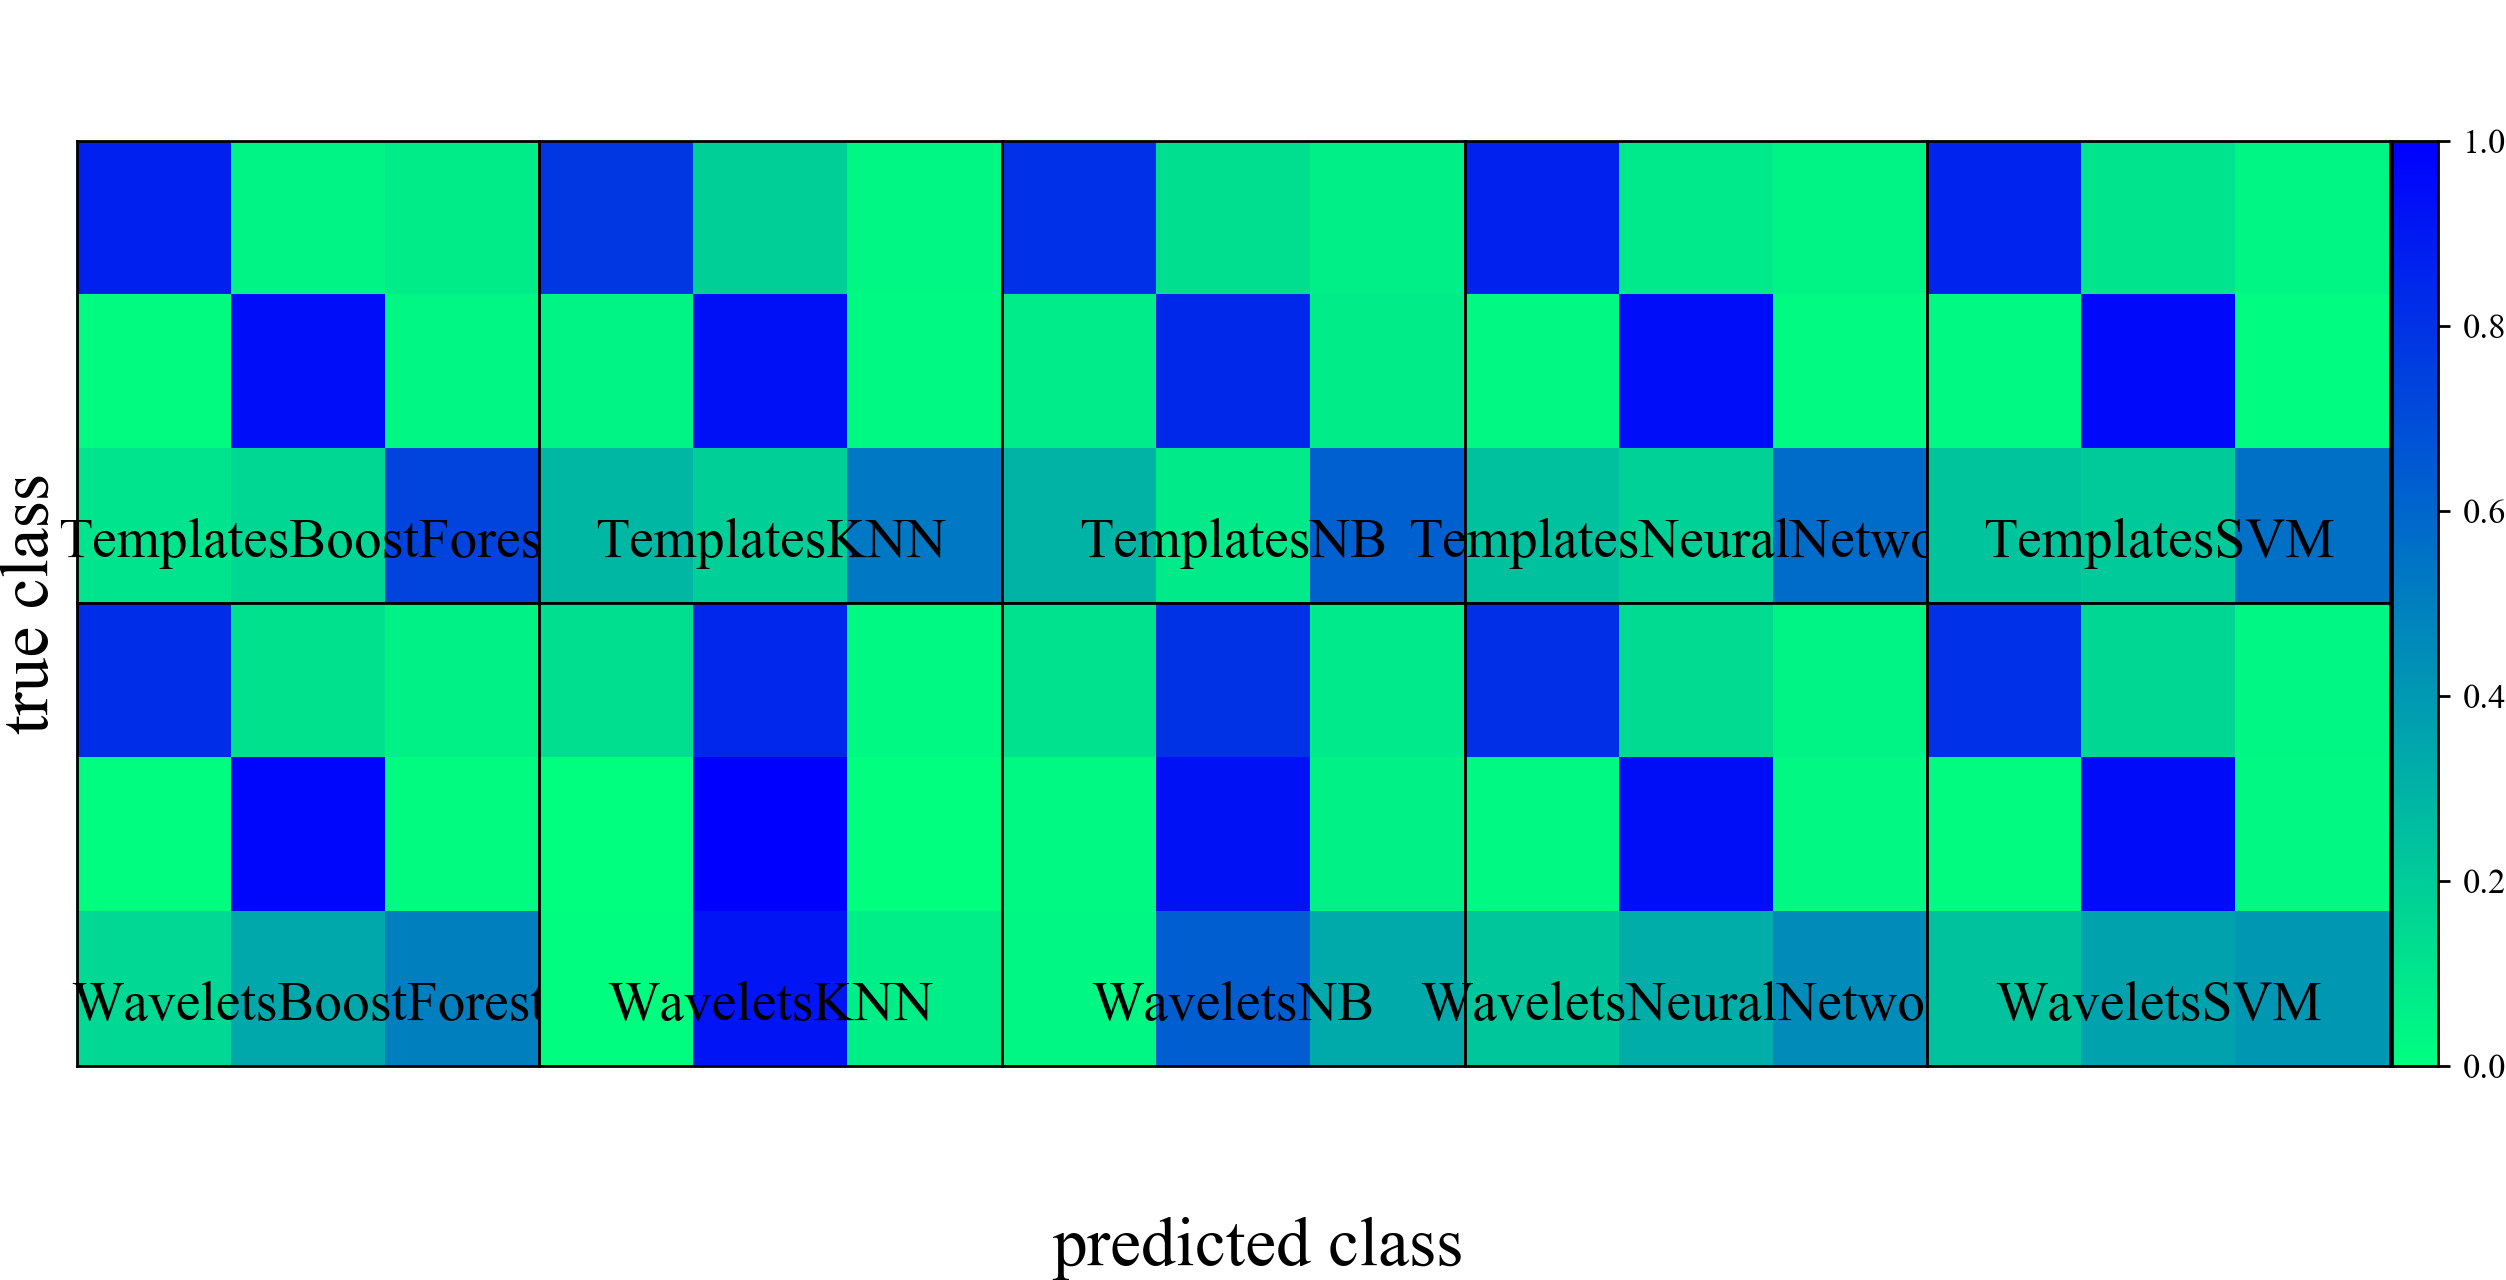
\includegraphics[width=\textwidth]{./fig/all_snphotcc_cm.png}
		\caption{Conditional probability matrices of the \citet{lochner_photometric_2016} methods applied to the \snphotcc\ dataset.
		Columns: the five machine learning methods of Boosted Decision Tree (BDT), K-Nearest Neighbors (KNN), Naive Bayes (NB), Neural Network (NN), and Support Vector Machine (SVM).
    Top row: five machine learning methods applied to template decompositions as features.
    Bottom row: the same five machine learning methods applied to wavelet decompositions as features.
		These CPMs derived from the dataset of a precursor lightcurve classification challenge by modern methods exhibit some of the systematics identified in Section~\ref{sec:mockdata} and Figure~\ref{fig:mock_cm}, particularly cruise control (WKNN, WNB), noisy (class Ibc in all but TBDT and WKNN), and perfect (class II in all).
		}
		\label{fig:snphotcc_cm}
	\end{center}
\end{figure*}

%\aim{This would be more meaningful if we were given the conditional probability matrices of actual submissions to \snphotcc\ and then checked whether the \plasticc\ metric would have designated a different winner.
%Also, it may be more interpretable if we instead use Ashish's conditional probability matrices that have more classes.}

In order to understand the performance of classifiers on simulated datasets approximating reality, we calculate the values of our metric candidates on representative classifiers of a precursor lightcurve classification challenge.
The Supernova Photometric Classification Challenge (\snphotcc) \citep{kessler_supernova_2010} focused on deterministically classifying a heterogenous population of supernovae into subclasses of SN Ia, SN II, and SN Ibc
The \snphotcc\ attracted diverse classification approaches, encompassing $\chi^{2}$ fits of the supernova lightcurves to publicly available templates \citep{nugent_kcorrections_2002}, physical models \citep{conley_sifto:_2008}, and empirical models, as well as alternatives to curve-fitting such as outlier identification on the training set Hubble diagram, dimensionality reduction, and clustering.
% TODO cite InCA?
% A general light curve shape (rather than one motivated by the physical differences between SNeIa and core collapse SNe) was assumed by some competitors and then a kernel density estimation was performed over the fit parameters, with various approaches employed including boosting over the feature space.
Machine learning was also employed, using features such as the light-curve slopes to produce a predictive model for the training data.
% TODO need citations of ML submissions to SNPhotCC
%, which are prone to bias given non-representativity of the test data and agnostic
\snphotcc\ attracted physically motivated template-based methods as well as those based on decomposition of the light curves into generic features at risk of neglecting available physical information.

Since the conclusion of the \snphotcc, the lightcurves became a testbed for a suite of machine learning classifiers.
We consider a collection of probabilistic classification methods, as presented in \citet{lochner_photometric_2016}, whose CPMs\footnote{The classifiers of \citet{lochner_photometric_2016} are indeed probabilistic but are reduced to confusion matrices via deterministic labels for this visualization and the science-motivated metric of Section~\ref{sec:science}.  In all other instances, the classification posteriors are used directly.} are shown in Figure~\ref{fig:snphotcc_cm}.
The set of classification algorithms includes template-based classification procedures, denoted as T, (\citet{sako_photometric_2011}, top row) and a wavelet decomposition, denoted as W, of the lightcurves to construct the features over which to classify (\citet{newling_statistical_2011}, bottom row), each paired with Boosted Decision Tree (BDT), K-Nearest Neighbors (KNN), Naive Bayes (NB), Neural Network (NN), and Support Vector Machine (SVM) machine learning algorithms (columns).
While the complexity of entries to the \snphotcc\ was greater than this subset, we use these examples to establish the behavior of our metrics on realistic classification submissions.

We draw attention to the marked presence of the systematics introduced in Section~\ref{sec:mockdata} in the CPMs of Figure~\ref{fig:snphotcc_cm}.
Note that the WNN and WNB methods both suffer from the cruise control systematic on SN II; it should come as no surprise that SN II are more prevalent in the \snphotcc\ dataset.
Nearly all the others exhibit classifications that are almost perfect for SN Ia, perfect for SN II, and noisy for SN Ibc.
A likely cause for this effect is that SN Ibc are poorly represented in training and template sets.
% \subsubsection{Unknown dataset}
% \label{sec:mystery}
%
% \begin{figure*}
% 	\begin{center}
% 		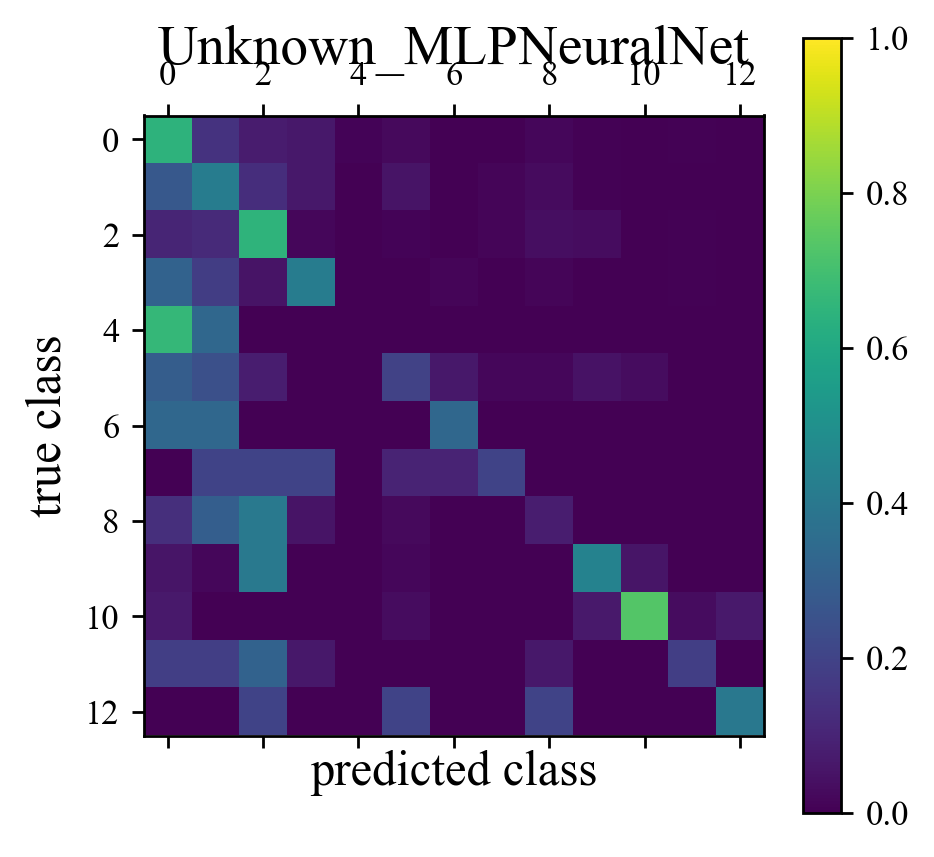
\includegraphics[width=0.3\textwidth]{./fig/Unknown_MLPNeuralNet_cm.png}
% 		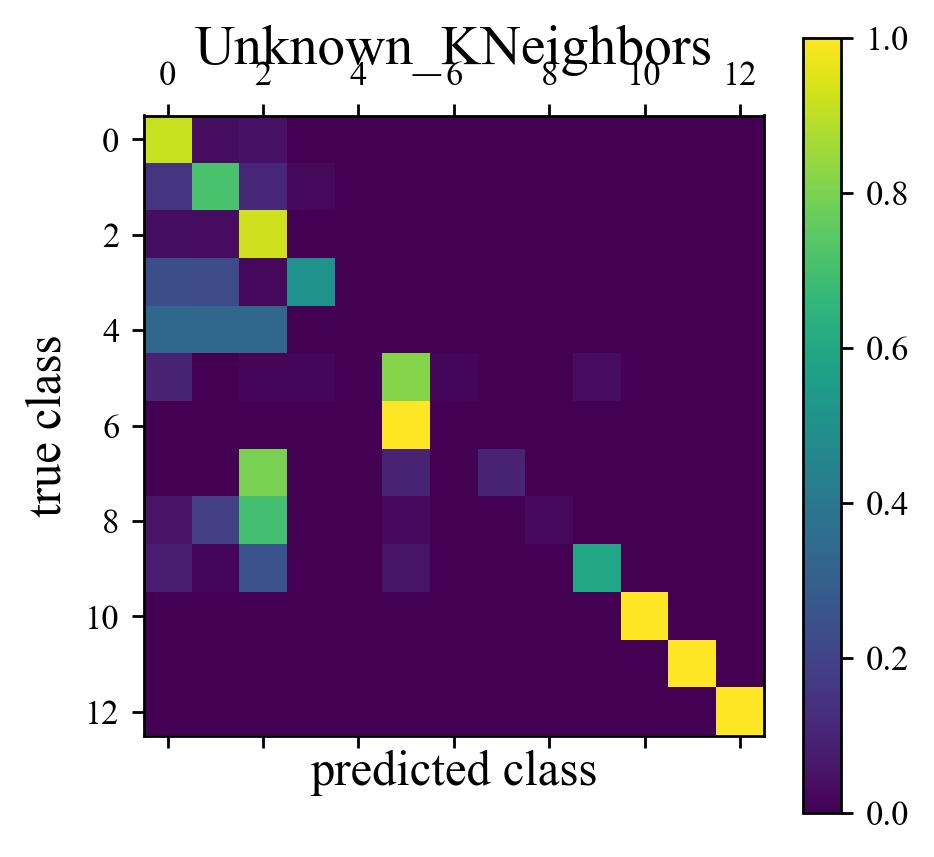
\includegraphics[width=0.3\textwidth]{./fig/Unknown_KNeighbors_cm.png}
% 		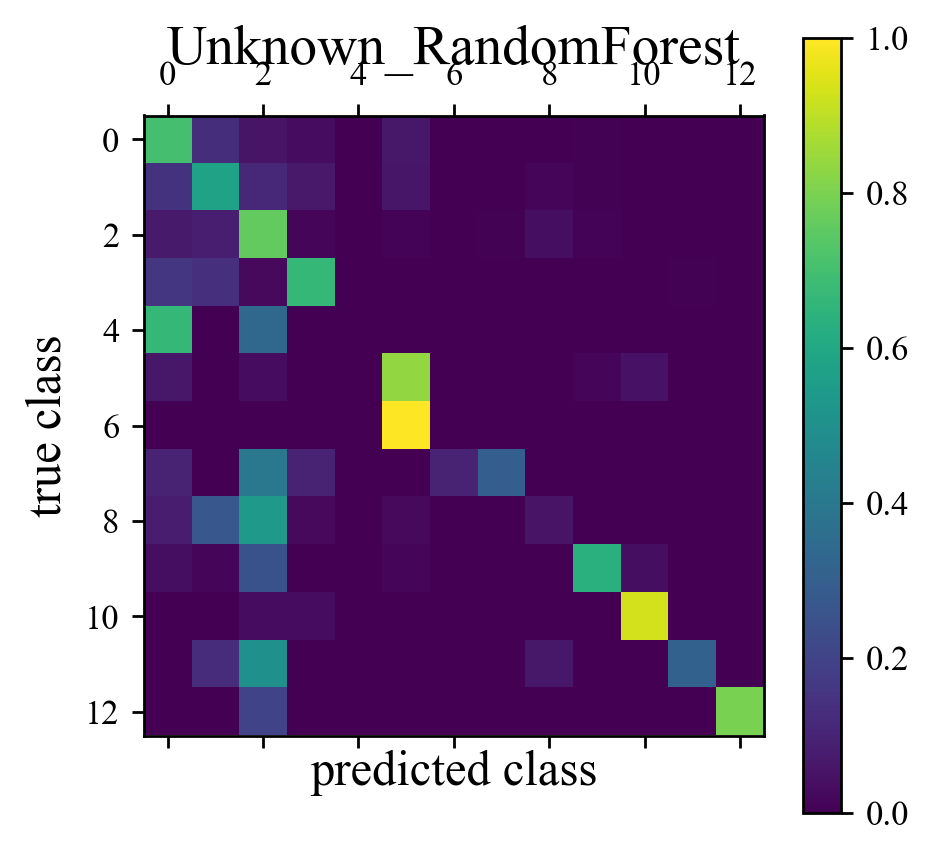
\includegraphics[width=0.3\textwidth]{./fig/Unknown_RandomForest_cm.png}
% 		\caption{}
% 		\label{fig:unknown_cm}
% 	\end{center}
% \end{figure*}
